\documentclass[tikz,border=4mm]{standalone}
\usepackage[T1]{fontenc}
\usepackage{helvet}
\renewcommand{\familydefault}{\sfdefault}
\usetikzlibrary{arrows.meta,positioning,fit,backgrounds}

\begin{document}
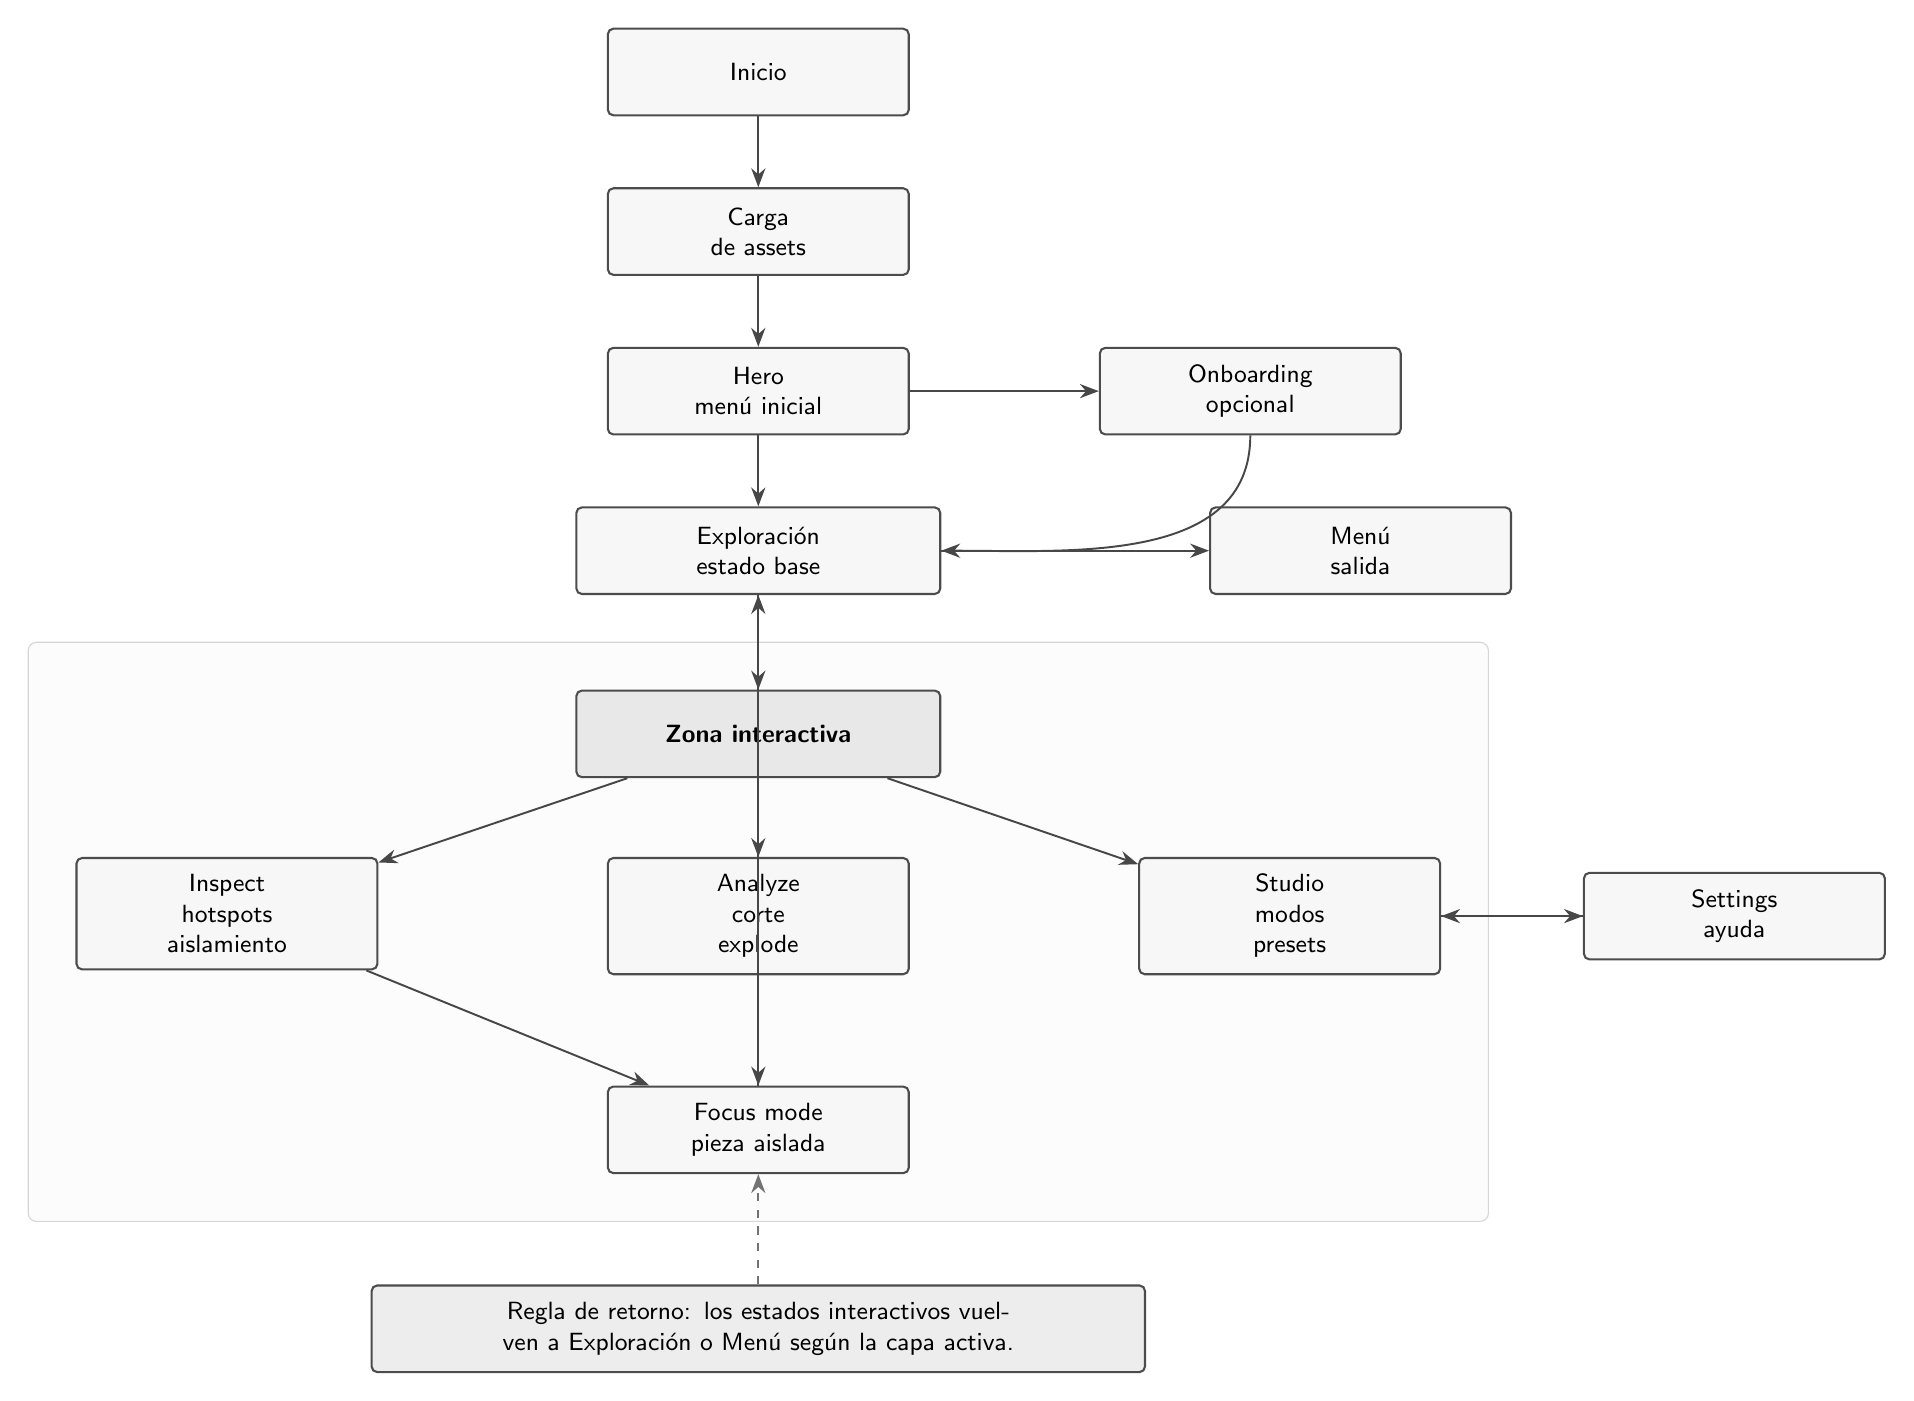
\begin{tikzpicture}[
  font=\sffamily\small,
  node distance=9mm and 12mm,
  box/.style={
    draw=black!70,
    rounded corners=2pt,
    line width=0.75pt,
    fill=black!3,
    align=center,
    inner sep=6pt,
    minimum height=11mm
  },
  state/.style={box, text width=34mm},
  wide/.style={box, text width=42mm},
  head/.style={box, fill=black!9, text width=42mm, font=\sffamily\bfseries\small},
  rule/.style={box, text width=94mm, fill=black!7},
  arrow/.style={-{Stealth[length=2.4mm]}, line width=0.7pt, draw=black!72},
  dashedarrow/.style={-{Stealth[length=2.4mm]}, line width=0.7pt, draw=black!55, dashed}
]

\node[state] (start) {Inicio};
\node[state, below=of start] (loading) {Carga\\de assets};
\node[state, below=of loading] (hero) {Hero\\men\'u inicial};
\node[state, right=24mm of hero] (intro) {Onboarding\\opcional};
\node[wide, below=of hero] (explore) {Exploraci\'on\\estado base};

\node[head, below=12mm of explore] (zonehead) {Zona interactiva};
\node[state, below left=10mm and 25mm of zonehead] (inspect) {Inspect\\hotspots\\aislamiento};
\node[state, below=10mm of zonehead] (analyze) {Analyze\\corte\\explode};
\node[state, below right=10mm and 25mm of zonehead] (studio) {Studio\\modos\\presets};
\node[state, below=14mm of analyze] (focus) {Focus mode\\pieza aislada};

\node[state, right=34mm of explore] (menu) {Men\'u\\salida};
\node[state, right=18mm of studio] (settings) {Settings\\ayuda};
\node[rule, below=14mm of focus] (rule) {Regla de retorno: los estados interactivos vuelven a Exploraci\'on o Men\'u seg\'un la capa activa.};

\begin{scope}[on background layer]
  \node[draw=black!16, rounded corners=3pt, fill=black!1,
    fit=(zonehead)(inspect)(analyze)(studio)(focus), inner sep=6mm] {};
\end{scope}

\draw[arrow] (start) -- (loading);
\draw[arrow] (loading) -- (hero);
\draw[arrow] (hero) -- (explore);
\draw[arrow] (hero) -- (intro);
\draw[arrow] (intro.south) to[out=-90,in=0] (explore.east);

\draw[arrow] (explore) -- (zonehead);
\draw[arrow] (zonehead) -- (inspect);
\draw[arrow] (zonehead) -- (analyze);
\draw[arrow] (zonehead) -- (studio);
\draw[arrow] (inspect) -- (focus);
\draw[arrow] (analyze) -- (focus);
\draw[arrow] (focus) -- (explore);

\draw[arrow] (explore) -- (menu);
\draw[arrow] (studio) -- (settings);
\draw[arrow] (settings) -- (studio);
\draw[dashedarrow] (rule) -- (focus);

\end{tikzpicture}
\end{document}
